\documentclass[10pt]{ctexart}
\usepackage{morelull}
\usepackage{enumerate}
\usepackage{bm}
\usepackage{makecell}
\usepackage{xcolor}
\usepackage{graphicx}
\usepackage{subfigure}
\usepackage{framed}%包中有添加文字背景色命令shaded
\colorlet{shadecolor}{MaterialBlue50}
\usepackage{tabularx}
\usepackage{multicol}  
\usepackage{multirow}
\usepackage{indentfirst}
\usepackage{amsmath,amssymb,amsthm,bm,bbding,pifont,dsfont}
\usepackage{mathtools}
\newcommand{\abs}[1]{\left| #1 \right|}
\usepackage{caption}
\captionsetup[figure]{labelfont={bf},labelformat={default},labelsep=period,name={图}}
%定义选择题选项
\newcommand{\onech}[4]{
\renewcommand\arraystretch{1.4}
\begin{tabularx}{\linewidth}{XXXX}
\setlength\tabcolsep{0pt}
(A) #1 & (B) #2 & (C) #3 & (D) #4 \\
\end{tabularx}
\unskip \unskip}
\newcommand{\twoch}[4]{
\renewcommand\arraystretch{1.4}
\begin{tabularx}{\linewidth}{XX}
\setlength\tabcolsep{0pt}
(A) #1 & (B) #2 \\
(C) #3 & (D) #4
\end{tabularx}
\unskip \unskip}

\title{模型研究系列 \quad 半角模型}
\author{一粒沙整理\\安徽省霍邱县龙潭中心校}
\date{\today}



\begin{document}
\maketitle
\tableofcontents


\section{什么是半角模型?}
所谓“半角模型”指的是题目中出现了两个角,小角等于大角的一半,故称为“半角模型”,有最普通的半角问题,但是多数“半角模型”问题都是特殊角之间的“半角模型”。常见的有“$30^\circ$与$60^\circ$”、“$45^\circ$与$90^\circ$”、“$60^\circ$与$120^\circ$”等类型。
\section{半角模型“破解”策略}
记住一句话:“\textcolor{red}{半角模型,必旋转}”
\begin{vuyi}

\kaishu (1)旋转角度通常为大角的角度;

(2)旋转后,往往涉及三点共线问题(须简单证明);

(3)旋转后,一般需要再证一对共旋转点的三角形全等(SAS).
\end{vuyi}
\section{“半角模型”的类型}
\subsection{$90^\circ +45^\circ$的半角模型}
\subsubsection{正方形中含半角及其变型}
如图,在正方形$ABCD$中,点$E,F$分别为边$BC,CD$上点,且$\angle EAF=45^\circ$,连接$EF$,$AH\perp EF$.
\begin{minipage}{0.3\textwidth}
	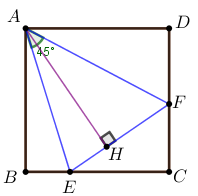
\includegraphics[scale=0.8]{figure/banjiao08}
\end{minipage}
\begin{minipage}{0.4\textwidth}
	结论\ding{192}:\textcolor{red}{$EF=BE+DF$};\\
	结论\ding{193}:\textcolor{red}{$\triangle CEF$的周长$C=2AB$};\\
	结论\ding{194}:\textcolor{red}{$AE$平分$\angle BEF$,$AF$平分$\angle DFE$};\\
	结论\ding{195}:\textcolor{red}{$AH=AB$};\\
	结论\ding{196}:\textcolor{red}{$S_{\triangle ABE}+S_{\triangle ADF}=S_{\triangle AEF}$}.
\end{minipage}


\begin{figure}[htp]
	 \begin{minipage}{0.5\linewidth}
		 \centering
		 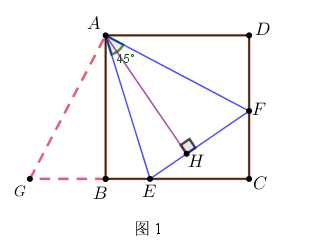
\includegraphics[scale=0.8]{figure/banjiao02.png}
		 \end{minipage}
	 \begin{minipage}{0.5\linewidth}
		 \centering
		 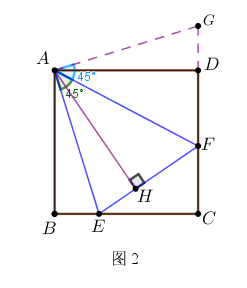
\includegraphics[scale=0.8]{figure/banjiao03.png}
		 \end{minipage}
	 \end{figure}
{\kaishu\color{blue}
证法\ding{192}:(\textcolor{red}{旋转法})

如图1,将$\triangle ADF$绕点$A$顺时针旋转$90^\circ$得到$\triangle ABG$.( 亦可旋转$\triangle ABE$)

易得$\triangle ADF\cong \triangle ABG \dashrightarrow AG=AF,DF=BG,\angle 1=\angle 2$;

再证$\triangle AEG\cong \triangle AEF\dashrightarrow EF=EG$;

综上:$EF=EG=BE+BG=BE+DF$.(结论\ding{192}得证)

$\triangle CEF$的周长$C=EF+CE+CF=BE+DF+CE+CF=BC+DC=2AB$.(结论\ding{193}得证)

由$\triangle AEG\cong \triangle AEEF\dashrightarrow AE$平分$\angle BEF$,同理可证$AF$平分$\angle AFE$.(结论\ding{194}得证)

利用结论\ding{194}易证$\triangle ABE\cong \triangle AHE(AAS)\dashrightarrow AB=AH$.(结论\ding{195}得证)

由\ding{192}易证$S_{\triangle ABE}+S_{\triangle ADF}=\dfrac{1}{2}EF\bm\cdot AB$,而$S_{\triangle AEF}=\dfrac{1}{2}EF\bm\cdot AH$,由\ding{195}易得$S_{\triangle ABE}+S_{\triangle ADF}=S_{\triangle AEF}$.(结论\ding{196}得证)


证法\ding{193}:(\textcolor{red}{截长补短法})

如图2,延长$CD$至点$G$使得$DG=BE$.

易证:$\triangle ABE\cong \triangle ADG(SAS)\dashrightarrow AE=AG,\angle GAF=45^\circ$;

易证:$\triangle AFE\cong \triangle AFG(SAS)\dashrightarrow EF=GF$;

综上:$EF=GF=GD+DF=BE+DF$.

其它结论证法同证法\ding{192}.}

进一步地,连接对角线后还可以得出下面8个结论:

如图,连接$BD$,分别交$AE,AF$于点$M,N$.

\vspace{2em}
\begin{minipage}{0.25\textwidth}
	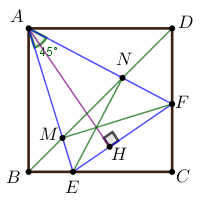
\includegraphics[scale=0.8]{figure/banjiao07.png}
\end{minipage}
\begin{minipage}{0.75\textwidth}
结论\ding{192}:\textcolor{red}{$MN^2=BM^2+DN^2$};\\
结论\ding{193}:\textcolor{red}{$2AM^2=BM^2+DM^2,2AN^2=DN^2+BN^2$};\\
结论\ding{194}:\textcolor{red}{$\triangle AEN$为等腰直角三角形,$\triangle AFM$为等腰直角三角形};\\
结论\ding{195}:\textcolor{red}{$\triangle ANM \sim \triangle DNF \sim \triangle BEM \sim \triangle AEF \sim \triangle BNA \sim \triangle DAM$};\\
结论\ding{196}:\textcolor{red}{$\sqrt{2}BN=AB+BE,\sqrt{2}DM=AD+DF$};\\
结论\ding{197}:\textcolor{red}{$\sqrt{2}DN=CE,\sqrt{2}BM=CF,\sqrt{2}MN=EF$};\\
结论\ding{198}:\textcolor{red}{$S_{\triangle AMN}=S_{\text{四边形}MNFE}$(即$S_{\triangle AMN}=\dfrac{1}{2}S_{AEF}$)};\\
结论\ding{199}:\textcolor{red}{$A,M,F,D$四点共圆;$A,B,E,N$四点共圆;$M,N,F,C,E$五点共圆}.
\end{minipage}
\vspace{2em}

下面我们来进行证明,对于结论\ding{192},我们用两种方法证明:

{\kaishu\color{blue}
\begin{minipage}[h]{0.4\textwidth}
	\centering
	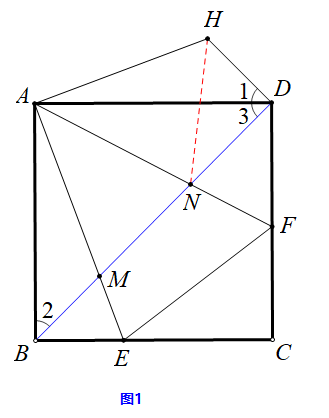
\includegraphics[width=0.7\textwidth]{figure/banjiao12}
\end{minipage}
\quad
\begin{minipage}[h]{0.6\textwidth}
证法\ding{192}:

将$\triangle AMB$逆时针$90^\circ$旋转到$\triangle AHD$,如图1.

则$\angle 2=\angle 1=\angle 3=45^\circ$

$\therefore \angle HDN=\angle 1+\angle 3=90^\circ$

$\therefore \triangle HDN$是直角三角形

$\because$易证$\triangle ANH\cong \triangle ANM$

$\therefore NH=NM$

在$Rt\triangle HDN$中,$HD^2+DN^2=HN^2$

又$\therefore NH=NM,HD=MB$

$\therefore BM^2+DN^2=MN^2$
\end{minipage}



\begin{minipage}[h]{0.4\textwidth}
	\centering
	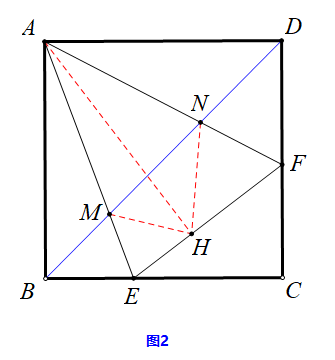
\includegraphics[width=0.7\textwidth]{figure/banjiao13}
\end{minipage}
\quad
\begin{minipage}[h]{0.6\textwidth}

证法\ding{193}:

过$A$作$AH$垂直$EF$于$H$,连接$MH,NH$,如图2.

易证,$\triangle ABM \cong \triangle AHM ,\triangle ADN \cong \triangle AHN$

$\therefore \angle AHM=\angle ABM=45^\circ,\angle AHN=\angle ADN=45^\circ$

$\therefore \angle MHN=90^\circ$

$MH^2+NH^2=MN^2$

又$\therefore MH=MB,NH=ND$

$\therefore BM^2+DN^2=MN^2$
\end{minipage}
}

结论\ding{193},我们也用两种方法予以证明,过程如下:

{\kaishu\color{blue}
\begin{minipage}[h]{0.6\textwidth}
证法\ding{192}:
	
将$\triangle AMB$逆时针$90^\circ$旋转到$\triangle AHD$,连接$MH$,如图1.

$\because AH=AM,\angle HAD+\angle DAN+\angle NAM=\angle HAM=90^\circ$

$\therefore HM=\sqrt{2}AM$

又$\therefore HD^2+DM^2=HM^2,HD=BM$


$\therefore BM^2+DM^2=HM^2=2AM^2$

同理$2AN^2=BN^2+DN^2$	

\end{minipage}
\quad
\begin{minipage}[h]{0.4\textwidth}
	\centering
	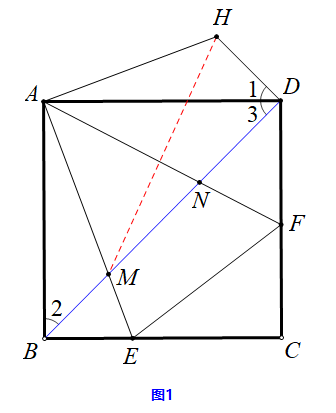
\includegraphics[width=0.6\textwidth]{figure/banjiao14}
\end{minipage}

\begin{minipage}[h]{0.6\textwidth}
	证法\ding{193}:
	
过$M$作$MP \perp AD$于$P$,$MH \perp AB$于$H$,如图2.

设$HM=HB=x,PM=PD=y$

$\therefore BM^2=2x^2,PM^2=2y^2$

又$\therefore AM^2=AH^2+HM^2=x^2+y^2$

$\therefore 2AM^2=BM^2+DM^2$

同理$2AN^2=BN^2+DN^2$		
\end{minipage}
\quad
\begin{minipage}[h]{0.4\textwidth}
	\centering
	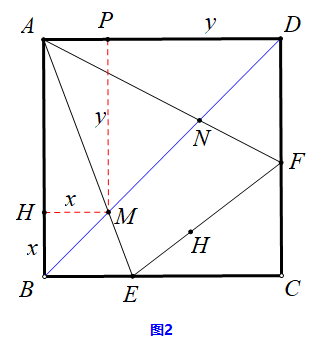
\includegraphics[width=0.6\textwidth]{figure/banjiao15}
\end{minipage}
}

结论\ding{194}的证明如下:

\begin{minipage}[h]{0.6\textwidth}
	证法\ding{193}:
	
	过$M$作$MP \perp AD$于$P$,$MH \perp AB$于$H$,如图2.
	
	设$HM=HB=x,PM=PD=y$
	
	$\therefore BM^2=2x^2,PM^2=2y^2$
	
	又$\therefore AM^2=AH^2+HM^2=x^2+y^2$
	
	$\therefore 2AM^2=BM^2+DM^2$
	
	同理$2AN^2=BN^2+DN^2$		
\end{minipage}
\quad
\begin{minipage}[h]{0.4\textwidth}
	\centering
	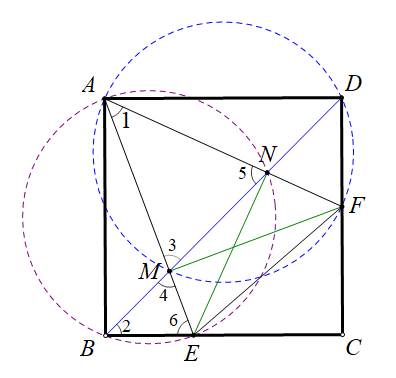
\includegraphics[width=0.7\textwidth]{figure/banjiao16}
\end{minipage}







\subsubsection{等腰直角三角形内含半角}
如图,在$\triangle ABC$中,$AB=AC,\angle BAC=90^\circ$,点$D,E$在$BC$上且$\angle DAE=45^\circ$.

性质:\ding{192}:$\triangle BAE \sim \triangle ADE \sim \triangle CDA$

\ding{193}:$BD^2+CE^2=DE^2$




\subsection{$120^\circ +60^\circ$的半角模型}
\begin{minipage}{0.6\textwidth}
	如图,已知$\triangle ABC$是正三角形,点$D$是$\triangle ABC$外一点,$DB=DC$且$\angle BDC=120^\circ,\angle EDF=60^\circ$,$DE,DF$分别交$AB,AC$于点$E,F$.
	此时可以推导出以下结论:
	
	结论\ding{192}:\textcolor{red}{$EF=BE+CF$};\\
	结论\ding{193}:\textcolor{red}{$C_{\triangle AEF}=2AB$}.
\end{minipage}\qquad\qquad
\begin{minipage}{0.4\textwidth}
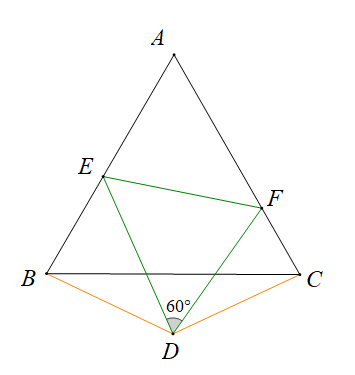
\includegraphics[scale=0.4]{figure/banjiao10.PNG}
\end{minipage}
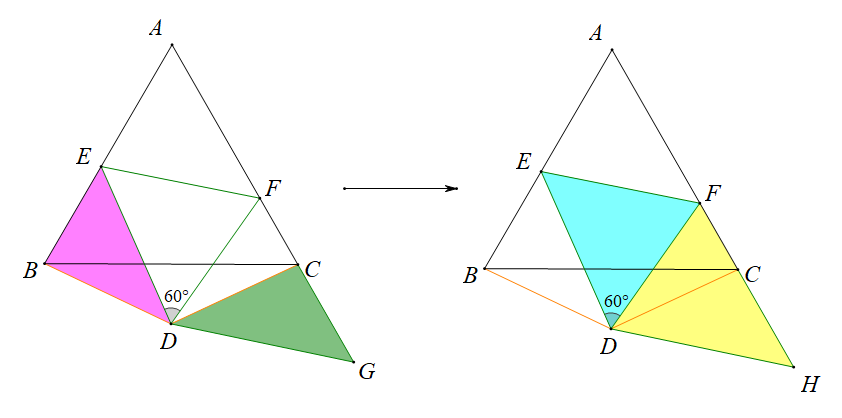
\includegraphics[scale=0.4]{figure/banjiao11.PNG}

\subsection{一般情况半角模型$\alpha +2\alpha$}




\section{习题演练}









\end{document}